% Tablas complementarias de los experimentos (movidas desde la seccion de experimentos).
\section{Additional tables}
\label{app:tables}

This appendix collects tables that support statements of Section~\ref{sec:experiments-bpp} but are not needed to follow it.

\begin{table}[t]
\centering
\small
\caption{Options of \texttt{BSG\_BPP} for each configuration.}
\label{tab:e-commands}
\begin{tabular}{@{}lp{9.5cm}@{}}
\toprule
Configuration & Options\\
\midrule
\cfgfast{} & \texttt{-T 4 -t 0.005 --harvest 10 --milp 30}\\
\cfgbal{} & \texttt{-T 20 -t 0.005 --harvest 10 --milp 60}\\
\cfgqual{} & \texttt{-T 100 --milp 100}\\
Industrial, $n\ge 500$ & \texttt{--no\_improve --kappa 1 -t 2 --support area}\\
Industrial, $n<500$ & \texttt{-T 10 -t 0.5 --kappa 1 --support area}\\
Industrial, $n<500$, improvement phase & \texttt{-T 30 --swo\_frac 0.3 --scratch --improve\_time 2 --kappa 1 --support area}\\
\bottomrule
\end{tabular}
\end{table}

\begin{table}[t]
\centering
\small\setlength{\tabcolsep}{3pt}
\caption{Budgets on the 240 original instances (classes 1 and 4--8), mean of three seeds. $T$, $T_{\mathrm{milp}}$: time limits of the search and
the recombination; $K$: harvest; $\tau=0.005$ s for \cfgfast{} and \cfgbal{}, and $\tau=0.02$ s for the two rows with $T=100$ s. The last column is the squeaky wheel
loop alone with a time limit equal to the mean time of the row.}
\label{tab:e-budget}
\begin{tabular}{@{}lrrrrrl@{}}
\toprule
 & $T$ & $T_{\mathrm{milp}}$ & $K$ & Bins & Time (s) & Squeaky wheel alone\\
\midrule
\cfgfast{} & 4 & 30 & 10 & $7256.7\pm 0.6$ & 6.7 & $7273.3\pm 1.5$ (6.6 s)\\
\cfgbal{} & 20 & 60 & 10 & $7256.0\pm 1.0$ & 25.9 & $7269.0\pm 1.0$ (24.3 s)\\
$T=100$, harvest & 100 & 100 & 10 & $7250.0\pm 1.0$ & 103.9 & $7266.3\pm 0.6$ (103.9 s)\\
\cfgqual{} & 100 & 100 & 0 & $7249.3\pm 1.2$ & 100.3 & $7266.3\pm 0.6$ (103.9 s)\\
\bottomrule
\end{tabular}
\end{table}

\begin{table}[t]
\centering
\small\setlength{\tabcolsep}{4pt}
\caption{Time per instance in seconds (wall-clock) over the 720 runs of each configuration on the 240 original instances. Limit: runs in which the MILP reached its time limit without a proof, over 720.}
\label{tab:e-time}
\begin{tabular}{@{}lrrrrrrrr@{}}
\toprule
Configuration & Mean & Median & 90th pct. & Maximum & Mean, $n=50$ & Mean, $n=200$ & Limit\\
\midrule
\cfgfast{} & 6.7 & 4.2 & 12.5 & 34.2 & 3.4 & 10.5 & 42\\
\cfgfast{} without harvest & 5.8 & 4.1 & 7.3 & 34.3 & 3.4 & 8.8 & 27\\
\cfgbal{} & 25.9 & 20.5 & 48.8 & 80.4 & 16.8 & 34.2 & 57\\
\cfgqual{} & 100.3 & 100.3 & 112.9 & 200.6 & 83.6 & 116.5 & 33\\
\bottomrule
\end{tabular}
\end{table}

\begin{table}[t]
\centering
\small\setlength{\tabcolsep}{4pt}
\caption{Contribution of the recombination inside the runs (240 original instances, three seeds). Before: total bins of the squeaky wheel loop (the incumbent that the
recombination starts from); After: total bins at the end; Better: instances in which the recombination saved a bin (the number of instances where it made the solution worse is zero in every case);
$p$: Wilcoxon signed-rank test per seed on the differences per instance; $t_{\mathrm{milp}}$: mean time of the recombination.}
\label{tab:e-within}
\begin{tabular}{@{}llrrrrrr@{}}
\toprule
Configuration & Seed & Before & After & Diff. & Better & $p$ & $t_{\mathrm{milp}}$ (s)\\
\midrule
\cfgfast{} & 1 & 7279 & 7257 & $-22$ & 22 & $3\cdot 10^{-6}$ & 2.7\\
 & 2 & 7278 & 7256 & $-22$ & 22 & $3\cdot 10^{-6}$ & 3.1\\
 & 3 & 7275 & 7257 & $-18$ & 18 & $2\cdot 10^{-5}$ & 2.7\\
\cfgfast{} without harvest & 1 & 7279 & 7270 & $-9$ & 9 & 0.0027 & 2.3\\
 & 2 & 7272 & 7264 & $-8$ & 8 & 0.0047 & 1.7\\
 & 3 & 7274 & 7264 & $-10$ & 10 & 0.0016 & 1.8\\
\cfgbal{} & 1 & 7271 & 7256 & $-15$ & 15 & 0.0001 & 7.0\\
 & 2 & 7271 & 7257 & $-14$ & 14 & 0.0002 & 7.2\\
 & 3 & 7270 & 7255 & $-15$ & 15 & 0.0001 & 7.1\\
\cfgqual{} & 1 & 7264 & 7248 & $-16$ & 16 & $6\cdot 10^{-5}$ & 6.6\\
 & 2 & 7266 & 7250 & $-16$ & 16 & $6\cdot 10^{-5}$ & 6.7\\
 & 3 & 7267 & 7250 & $-17$ & 17 & $4\cdot 10^{-5}$ & 7.6\\
\bottomrule
\end{tabular}
\end{table}

\begin{table}[t]
\centering
\footnotesize\setlength{\tabcolsep}{3pt}
\caption{Blind set (128 instances, three seeds). Bins: mean and standard deviation of the total over the seeds. Pool: mean number of columns. MILP improves, Proven and Unproven: number of runs (of 384, three seeds)
in which the MILP found a solution with fewer bins than the squeaky wheel loop, in which the run ends with a proof that the pool has no better solution (by the LP or by the MILP), and in which the MILP reached its limit without a proof.
MILP time: mean per run. ``plain MILP'': warm start only, without the LP proof and the fixing (no proof is recorded).}
\label{tab:e-recomb}
\begin{tabular}{@{}lrrrrrrr@{}}
\toprule
Configuration & Bins & Time (s) & Pool & MILP improves & Proven & Unproven & MILP time (s)\\
\midrule
Squeaky wheel alone, $T=26$ s & $3893.0\pm 1.0$ & 25.3 & --- & --- & --- & --- & ---\\
\cfgfast{} without harvest & $3893.0\pm 0.0$ & 5.8 & 466 & 28 & 371 & 13 & 1.9\\
\cfgfast{} & $3884.0\pm 1.0$ & 6.3 & 3524 & 54 & 368 & 16 & 2.4\\
\cfgbal{} & $3882.0\pm 1.0$ & 24.8 & 12052 & 36 & 363 & 21 & 5.4\\
\cfgbal{}, plain MILP & $3883.7\pm 0.6$ & 35.3 & 12029 & 30 & --- & --- & 15.9\\
\bottomrule
\end{tabular}
\end{table}

\begin{figure}[t]
\centering
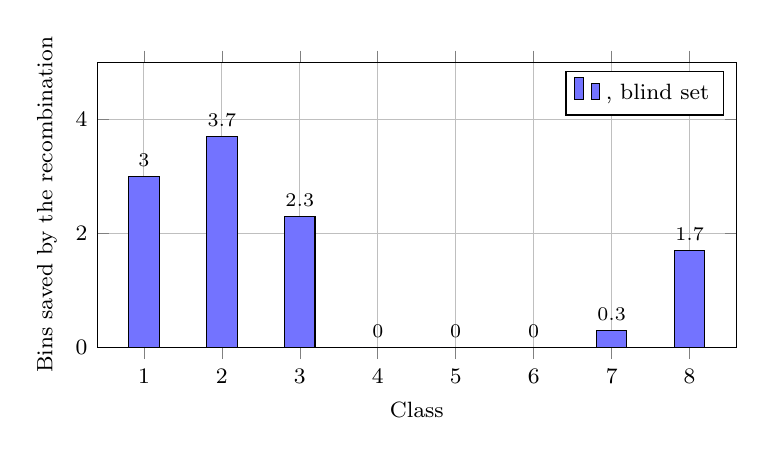
\begin{tikzpicture}
\begin{axis}[width=0.8\textwidth,height=5.2cm,ybar,bar width=11pt,xmin=0.4,xmax=8.6,ymin=0,ymax=5,xtick={1,2,3,4,5,6,7,8},
  xlabel={Class},ylabel={Bins saved by the recombination},grid=major,legend style={font=\footnotesize,at={(0.98,0.97)},anchor=north east},
  tick label style={font=\footnotesize},label style={font=\footnotesize},nodes near coords,every node near coord/.append style={font=\scriptsize}]
\addplot[fill=blue!55,bar shift=0pt] coordinates {(1,3.0) (2,3.7) (3,2.3) (4,0) (5,0) (6,0) (7,0.3) (8,1.7)};
\addlegendentry{\cfgbal{}, blind set}
\end{axis}
\end{tikzpicture}
\caption{Bins saved by the recombination of \cfgbal{} with respect to the squeaky wheel alone with the same time, by class (blind set; mean over the seeds; sums over the 16 instances of the class). Classes 4, 5 and 6 gain nothing.}
\label{fig:e-class}
\end{figure}

\begin{table}[t]
\centering
\small\setlength{\tabcolsep}{4pt}
\caption{Time per bin $\tau$ and profit exponent $\kappa$ on the industrial instances ($n\ge 500$, 80 instances, construction alone, support 70\%): total bins (mean and standard deviation over three seeds) and mean time per instance. The lower bound sums to 651.}
\label{tab:e-indkappa}
\begin{tabular}{@{}lrr@{}}
\toprule
Configuration & Bins & Time (s)\\
\midrule
$\kappa=1$, $\tau=2$ s (used) & $722.0\pm 1.0$ & 18.0\\
$\kappa=2$, $\tau=2$ s & $733.0\pm 1.0$ & 18.4\\
$\kappa=2$, $\tau=0.02$ s (default for MPV) & $825.7\pm 1.2$ & 0.5\\
\bottomrule
\end{tabular}
\end{table}

\begin{table}[t]
\centering
\small\setlength{\tabcolsep}{4pt}
\caption{Sensitivity to the parameters of the squeaky wheel loop and of the harvest: 72 original instances (classes 1 and 4--8, sizes 50 to 200, instances 1 to 3), configuration \cfgfast{} with one parameter changed, three seeds, four runs in parallel.
Total: mean and standard deviation over the seeds; Diff.: difference with the default, in bins; Better/worse: number of instances in which the variant is better or worse than the default (means over the seeds); $p$: Wilcoxon signed-rank test on those means; time: mean per instance.}
\label{tab:e-sens}
\begin{tabular}{@{}llrrrrr@{}}
\toprule
Parameter & Value & Total & Diff. & Better/worse & $p$ & Time (s)\\
\midrule
 & default & $2172.7\pm 1.2$ & --- & --- & --- & 7.0\\
\midrule
$\rho$ & 0.1 & $2171.3\pm 2.1$ & $-1.3$ & 5/3 & 0.12 & 6.3\\
 & 0.6 & $2171.3\pm 1.5$ & $-1.3$ & 4/1 & 0.13 & 6.9\\
 & 1.0 & $2172.0\pm 1.0$ & $-0.7$ & 3/2 & 0.34 & 7.1\\
$\sigma$ & 0 & $2170.7\pm 0.6$ & $-2.0$ & 4/0 & 0.066 & 6.4\\
 & 0.02 & $2171.0\pm 0.0$ & $-1.7$ & 4/0 & 0.066 & 6.8\\
 & 0.1 & $2172.3\pm 1.5$ & $-0.3$ & 2/1 & 0.59 & 7.0\\
 & 0.2 & $2176.0\pm 1.7$ & $+3.3$ & 2/8 & 0.016 & 8.3\\
Fraction of bins & 0.05 & $2170.7\pm 1.2$ & $-2.0$ & 4/1 & 0.14 & 6.1\\
 & 0.2 & $2171.0\pm 1.0$ & $-1.7$ & 4/1 & 0.10 & 6.9\\
 & 0.3 & $2171.7\pm 1.2$ & $-1.0$ & 3/2 & 0.42 & 7.2\\
$K$ & 1 & $2171.0\pm 0.0$ & $-1.7$ & 6/2 & 0.40 & 6.0\\
 & 3 & $2171.3\pm 1.2$ & $-1.3$ & 3/1 & 0.27 & 6.4\\
 & 30 & $2172.0\pm 1.0$ & $-0.7$ & 2/1 & 0.29 & 7.2\\
$\theta$ & 0.8 & $2170.7\pm 1.5$ & $-2.0$ & 6/1 & 0.047 & 6.7\\
 & 0.9 & $2170.7\pm 1.5$ & $-2.0$ & 5/1 & 0.14 & 6.8\\
 & 0.99 & $2171.0\pm 1.0$ & $-1.7$ & 4/1 & 0.10 & 6.3\\
$\tau$ (s) & 0.002 & $2171.0\pm 1.0$ & $-1.7$ & 4/1 & 0.10 & 7.5\\
 & 0.01 & $2172.3\pm 0.6$ & $-0.3$ & 3/2 & 0.79 & 6.7\\
 & 0.02 & $2177.0\pm 1.0$ & $+4.3$ & 1/9 & 0.041 & 5.9\\
\bottomrule
\end{tabular}
\end{table}

\begin{table}[t]
\centering
\small\setlength{\tabcolsep}{4pt}
\caption{Industrial instances with 70\% support on every box: total bins over 80 instances ($n\ge 500$ and $n<500$), mean and standard deviation over three seeds (current version of the code, four runs in parallel); time per instance in brackets.
$T$: time limit of the squeaky wheel loop; $\tau$: time per bin; ``recomb.'': harvest ($K=10$) and partitioning recombination. LCGA: sum over the cells of five times the mean of the cell \citep{Elhedhli2019}.}
\label{tab:e-indsw}
\begin{tabular}{@{}lrr@{}}
\toprule
Configuration & Bins & Time (s)\\
\midrule
\multicolumn{3}{@{}l}{$n\ge 500$ (80 instances)}\\
Construction alone, $\tau=2$ s & $722.0\pm 1.0$ & 17.9\\
Loop, $T=18$ s, $\tau=0.2$ s & $756.0\pm 1.7$ & 18.0\\
Loop, $T=18$ s, $\tau=0.5$ s & $727.7\pm 0.6$ & 17.2\\
Loop and recomb., $T=18$ s, $\tau=0.2$ s & $755.3\pm 2.5$ & 18.1\\
Loop and recomb., $T=18$ s, $\tau=0.5$ s & $729.3\pm 1.5$ & 17.4\\
Loop, $T=60$ s, $\tau=0.5$ s & $722.7\pm 0.6$ & 49.7\\
Loop and recomb., $T=60$ s, $\tau=0.5$ s & $722.7\pm 0.6$ & 49.4\\
LCGA & 768.0 & 608\\
\midrule
\multicolumn{3}{@{}l}{$n<500$ (80 instances)}\\
Construction alone, $\tau=2$ s & $115.0\pm 0.0$ & 2.4\\
Loop, $T=10$ s, $\tau=0.5$ s & $110.7\pm 0.6$ & 1.4\\
Loop and recomb., $T=10$ s, $\tau=0.5$ s & $110.7\pm 0.6$ & 1.4\\
Improvement phase, $T=30$ s & $112.7\pm 1.5$ & 3.5\\
LCGA & 115.0 & 20\\
\bottomrule
\end{tabular}
\end{table}

\begin{table}[t]
\centering
\small\setlength{\tabcolsep}{4pt}
\caption{Effect of the harvest at the budget of \cfgfast{} ($T=4$ s, $\tau=0.005$ s, $T_{\mathrm{milp}}=30$ s; 240 original instances).}
\label{tab:e-harvest}
\begin{tabular}{@{}lrrrrr@{}}
\toprule
 & Seed 1 & Seed 2 & Seed 3 & Mean $\pm$ sd & Time (s)\\
\midrule
Without harvest & 7270 & 7264 & 7264 & $7266.0\pm 3.5$ & 5.8\\
With harvest ($K=10$) & 7257 & 7256 & 7257 & $7256.7\pm 0.6$ & 6.7\\
Difference & $-13$ & $-8$ & $-7$ & $-9.3$ & $+0.9$\\
$p$ (Wilcoxon, per seed) & 0.0003 & 0.021 & 0.035 & & \\
\bottomrule
\end{tabular}
\end{table}

\begin{table}[t]
\centering
\small\setlength{\tabcolsep}{4pt}
\caption{Criteria of support (industrial instances, $n\ge 500$, 80 instances, construction alone, $\kappa=1$, $\tau=2$ s): total bins (mean and standard deviation over three seeds), mean time per instance, and support of the solutions (means over the seeds). Support: percentage of the base area resting on boxes.}
\label{tab:e-support}
\begin{tabular}{@{}lrrrrr@{}}
\toprule
Criterion & Bins & Time (s) & Mean support & Boxes with $\ge 70\%$ & Boxes fully supported\\
\midrule
None & $707.0\pm 1.7$ & 17.2 & 80.2\% & 77.3\% & 26.8\%\\
50\% of the base & $720.0\pm 0.0$ & 17.6 & 88.8\% & 87.4\% & 30.2\%\\
70\% of the base (used) & $721.7\pm 1.2$ & 18.0 & 91.4\% & 100\% & 30.7\%\\
85\% of the base & $788.0\pm 1.7$ & 19.2 & 95.0\% & 100\% & 34.8\%\\
Full support & $1297.3\pm 2.5$ & 31.6 & 100\% & 100\% & 100\%\\
\bottomrule
\end{tabular}
\end{table}
